% =====================================================================
% PRJ-23 - Aircraft Preliminary Design
% Homework 04 - Analise Aerodinamica (AVL)
% Grupo NJ-0502 - Instituto Tecnologico de Aeronautica
% Compilar com: python compila.py   (ou pdflatex main.tex duas vezes)
% =====================================================================
\documentclass[11pt,a4paper]{article}

\usepackage[utf8]{inputenc}
\usepackage[T1]{fontenc}
\usepackage[brazil]{babel}
\usepackage{lmodern}
\usepackage{amsmath,amssymb}
\usepackage{graphicx}
\usepackage{booktabs}
\usepackage{longtable}
\usepackage{float}
\usepackage{xcolor}
\usepackage{microtype}
\usepackage{enumitem}
\usepackage[margin=2.4cm]{geometry}
\usepackage[font=small,labelfont=bf]{caption}
\usepackage{fancyhdr}
\usepackage{pdflscape}
\usepackage[colorlinks=true,linkcolor=black,citecolor=black,urlcolor=blue!60!black]{hyperref}

\pagestyle{fancy}
\fancyhf{}
\fancyhead[L]{\small PRJ-23 --- Projeto Preliminar de Aeronave}
\fancyhead[R]{\small Lab 04 --- Análise Aerodinâmica}
\fancyfoot[C]{\thepage}
\renewcommand{\headrulewidth}{0.4pt}

\newcommand{\code}[1]{\texttt{\small #1}}

\begin{document}

\begin{titlepage}
  \centering
  \vspace*{1cm}

  {\Large \textbf{Instituto Tecnológico de Aeronáutica}} \\[0.4cm]
  {\large Departamento de Engenharia Aeronáutica} \\[1.5cm]

  \rule{\linewidth}{1pt} \\[0.4cm]
  {\LARGE \textbf{PRJ-23 --- Laboratório 04}} \\[0.3cm]
  {\Large NJ-0502} \\[0.3cm]
  \rule{\linewidth}{1pt} \\[2cm]

  \begin{tabular}{rl}
    \textbf{Integrantes:}  & Bruno Pimentel Santos \\
                           & Douglas Rodrigues Cabral \\
                           & Emanuel Garcia Alarcon \\
                           & Gabriel Souza Bonanni \\
                           & Joao Pedro Cruz Magalhaes \\
                           & Yuri Miranda Peres \\[0.6cm]
    \textbf{Professor:}    & Maj Eng Ney Rafael Secco \\[0.6cm]
    \textbf{Data:}         & 25 de setembro de 2026 \\
  \end{tabular}

  \vfill
  {\small São José dos Campos, 2026}
\end{titlepage}

\newpage

% ---------------------------------------------------------------------
% Este arquivo monta apenas as seções já produzidas. Acrescente os
% \input das demais seções (itens 2.1 a 2.3, 2.6 a 2.8 e a Seção 3 de
% derivadas de estabilidade) conforme forem ficando prontas, e registre
% os nomes correspondentes na lista SECOES de compila.py.
% ---------------------------------------------------------------------

% =====================================================================
% Lab 04 --- Item 2.4: metodo da secao critica
% Incluido por main.tex. Tabelas em tex_q4/ e figuras em
% resultados_q4/ (mesmo nivel que este arquivo e o main.tex).
% Codigos em secao_critica/.
% =====================================================================
% gerado por q4_secao_critica.py
\newcommand{\scAfilamento}{0.20}
\newcommand{\scAlphaAftLivre}{5.98}
\newcommand{\scAlphaAftTrim}{5.98}
\newcommand{\scAlphaAsa}{10.48}
\newcommand{\scAlphaCorrAftLivre}{11.48}
\newcommand{\scAlphaCorrAftTrim}{11.48}
\newcommand{\scAlphaCorrFwdLivre}{11.48}
\newcommand{\scAlphaCorrFwdTrim}{11.49}
\newcommand{\scAlphaFwdLivre}{5.98}
\newcommand{\scAlphaFwdTrim}{5.99}
\newcommand{\scAlphaNormAftLivre}{7.24}
\newcommand{\scAlphaNormAftTrim}{7.24}
\newcommand{\scAlphaNormFwdLivre}{7.24}
\newcommand{\scAlphaNormFwdTrim}{7.25}
\newcommand{\scCLmaxAftLivre}{0.877}
\newcommand{\scCLmaxAftTrim}{0.882}
\newcommand{\scCLmaxCorrAftLivre}{1.347}
\newcommand{\scCLmaxCorrAftTrim}{1.347}
\newcommand{\scCLmaxCorrFwdLivre}{1.334}
\newcommand{\scCLmaxCorrFwdTrim}{1.304}
\newcommand{\scCLmaxDT}{1.304}
\newcommand{\scCLmaxFwdLivre}{0.864}
\newcommand{\scCLmaxFwdTrim}{0.854}
\newcommand{\scCLmaxNormAftLivre}{0.986}
\newcommand{\scCLmaxNormAftTrim}{0.990}
\newcommand{\scCLmaxNormFwdLivre}{0.974}
\newcommand{\scCLmaxNormFwdTrim}{0.958}
\newcommand{\scClmaxDT}{1.773}
\newcommand{\scClmaxPonta}{1.526}
\newcommand{\scClmaxPontaN}{1.718}
\newcommand{\scClmaxRaiz}{1.783}
\newcommand{\scClmaxRaizN}{2.025}
\newcommand{\scCordaPonta}{2.00}
\newcommand{\scCordaRaiz}{10.02}
\newcommand{\scCosL}{0.8172}
\newcommand{\scDeAftLivre}{+0.00}
\newcommand{\scDeAftTrim}{+0.97}
\newcommand{\scDeFwdLivre}{+0.00}
\newcommand{\scDeFwdTrim}{-1.95}
\newcommand{\scEtaAftLivre}{0.907}
\newcommand{\scEtaAftTrim}{0.907}
\newcommand{\scEtaAil}{0.68}
\newcommand{\scEtaFlap}{0.66}
\newcommand{\scEtaFwdLivre}{0.907}
\newcommand{\scEtaFwdTrim}{0.907}
\newcommand{\scEtaPlatFim}{0.93}
\newcommand{\scEtaPlatIni}{0.79}
\newcommand{\scEtaSlat}{0.90}
\newcommand{\scFatorCarga}{1.20}
\newcommand{\scInvCosDois}{1.4975}
\newcommand{\scItAft}{-1.959}
\newcommand{\scItFwd}{-3.429}
\newcommand{\scIw}{4.5}
\newcommand{\scMach}{0.253}
\newcommand{\scPerdaCLAft}{-0.6}
\newcommand{\scPerdaCLFwd}{1.2}
\newcommand{\scRazaoColunas}{1.5040}
\newcommand{\scRazaoColunasMax}{1.5046}
\newcommand{\scRazaoColunasMin}{1.5039}
\newcommand{\scRazaoDT}{68}
\newcommand{\scRemac}{4.01}
\newcommand{\scSweep}{35.2}
\newcommand{\scTcPonta}{0.080}
\newcommand{\scTcRaiz}{0.160}
\newcommand{\scVdois}{86.0}
\newcommand{\scXcgAft}{29.91}
\newcommand{\scXcgFwd}{28.75}


\section{Item 4 --- Método da seção crítica e $C_{L\,max}$ de asa limpa}
\label{sec:secao-critica}

\subsection{Condição de voo e dados de entrada}

O estudo é feito na condição de baixa velocidade pedida pelo enunciado. Em vez
do valor genérico $M=0{,}2$ do roteiro, adotou-se a velocidade de segurança de
decolagem da própria aeronave,
\begin{equation}
  V_2 = 1{,}2\,V_s = \scVdois~\mathrm{m/s}
  \quad\Longrightarrow\quad
  M = \scMach,
  \qquad
  Re_{\mathrm{MAC}} = \scRemac \times 10^{7},
\end{equation}
ao nível do mar, calculada com $W_0$ e o $C_{L\,max}$ de decolagem do
\code{designTool}. A escolha não é estética: é exatamente o par $(Re, M)$ em que
o $c_{\ell\,max}$ do perfil otimizado foi levantado no XFOIL durante o Lab~03,
de modo que o limite usado aqui é o mesmo daquele relatório e não há
inconsistência de condição entre as duas tarefas. A diferença em relação a
$M=0{,}2$ é irrelevante para o AVL, que só usa o Mach na correção de
Prandtl--Glauert.

Todas as superfícies de alta sustentação ficam neutras (asa limpa: \code{flap},
\code{slat} e \code{aileron} em zero). A incidência de empenagem é a determinada
no item~3, $i_t = \scItFwd^\circ$ para o arquivo \code{fwd.avl} e
$i_t = \scItAft^\circ$ para o \code{aft.avl}.

\paragraph{Atenção ao referencial de $\alpha$.}
Desde o item~3 a superfície \code{Wing} dos arquivos \code{.avl} carrega o
cartão \code{ANGLE} com $i_w = \scIw^\circ$, escolhido para a fuselagem voar
nivelada no ponto de projeto. Com isso o $\alpha$ que o AVL reporta é o
\textbf{ângulo da fuselagem}, não o da asa: a asa vê $\alpha + i_w$. Todos os
$\alpha_{max}$ desta seção estão no referencial da fuselagem --- que é o que
interessa para \emph{tailstrike} e para a atitude de aproximação --- e o ângulo
de ataque visto pela asa no estol é
$\alpha_{max} + \scIw^\circ = \scAlphaAsa^\circ$.

\subsection{Limite de $c_{\ell\,max}$ ao longo da envergadura}

A asa da NJ-0502 tem afilamento $\lambda = \scAfilamento$, com corda de
\scCordaRaiz~m na raiz e \scCordaPonta~m na ponta. O Reynolds local varia
portanto por um fator de cinco, e o $c_{\ell\,max}$ do perfil não pode ser
tratado como constante. Rodou-se o XFOIL (mesmo tratamento de painéis do
Lab~03: \code{PPAR} com $T=0{,}45$ e $N=200$) para sete valores de corda,
obtendo-se
\begin{equation}
  c_{\ell\,max} = \scClmaxRaiz \ \text{na raiz}
  \qquad\longrightarrow\qquad
  c_{\ell\,max} = \scClmaxPonta \ \text{na ponta},
\end{equation}
conforme a Tab.~\ref{tab:clmax-perfil} e a Fig.~\ref{fig:clmax-perfil}. Note-se
que o valor na MAC reproduz o $c_{\ell\,max}$ do Lab~03 e é coerente com o
\code{clmax\_w} $=\scClmaxDT$ usado como entrada do \code{designTool}.

\begin{table}[H]
\centering
\caption{$c_{\ell\,max}$ do perfil \code{airfoil\_lab03.dat} em função da corda
local (XFOIL, $M=\scMach$). A coluna $\eta$ indica a estação da asa
trapezoidal com aquela corda.}
\label{tab:clmax-perfil}
\begin{tabular}{rrrrr}
\toprule
$c$ [m] & $\eta$ & $Re$ [$\times 10^{7}$] & $c_{\ell\,max}$ & $\alpha_{c_{\ell max}}$ [$^\circ$] \\
\midrule
10.02 & 0.00 & 5.83 & 1.783 & 17.00 \\
8.00 & 0.25 & 4.65 & 1.759 & 17.00 \\
6.90 & 0.39 & 4.01 & 1.737 & 17.00 \\
5.00 & 0.63 & 2.91 & 1.697 & 16.75 \\
4.00 & 0.75 & 2.33 & 1.646 & 16.75 \\
3.00 & 0.88 & 1.74 & 1.618 & 15.75 \\
2.00 & 1.00 & 1.17 & 1.526 & 15.25 \\
\bottomrule
\end{tabular}

\end{table}

\begin{figure}[H]
\centering
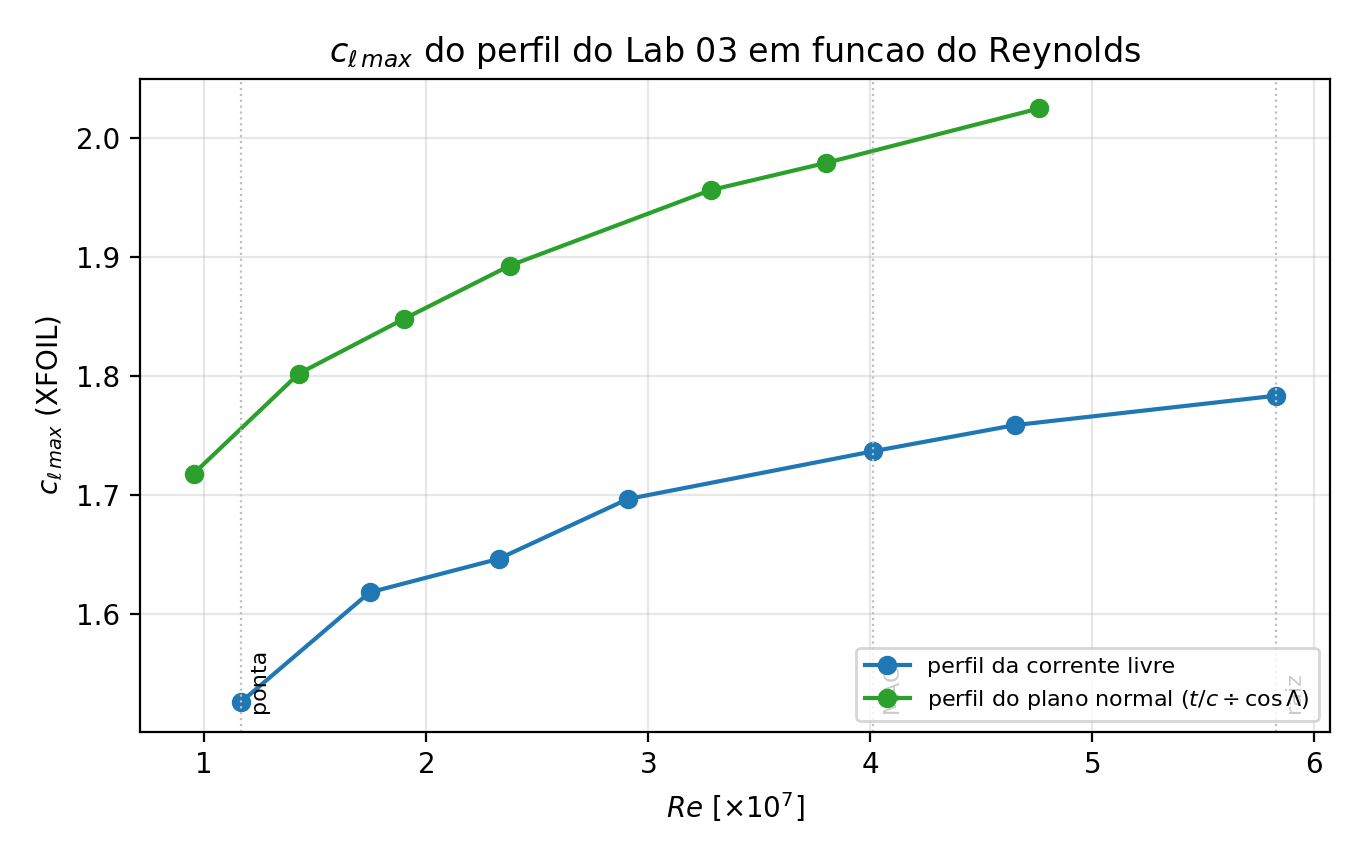
\includegraphics[width=0.66\textwidth]{resultados_q4/clmax_perfil_Re.png}
\caption{$c_{\ell\,max}$ do perfil em função do Reynolds, nos dois planos de
referência discutidos na Seção~\ref{sec:sc-criterio}.}
\label{fig:clmax-perfil}
\end{figure}

\subsection{Critério de estol e leitura das colunas do AVL}
\label{sec:sc-criterio}

O comando \code{fs} do AVL imprime, para cada faixa, duas colunas de
coeficiente de sustentação de seção: \code{cl}, referida à corda e à pressão
dinâmica da corrente livre, e \code{cl\_norm}, referida ao plano normal ao bordo
de ataque. Verificou-se numericamente que a razão entre as duas é praticamente
constante ao longo da envergadura (entre \scRazaoColunasMin{} e
\scRazaoColunasMax{}, mediana \scRazaoColunas) e coincide, a menos de $0{,}2\%$,
com $1/\cos^{2}\Lambda = 1/\cos^{2}\scSweep^\circ = \scInvCosDois$; ou seja,
\begin{equation}
  c_\ell^{\,norm} = \frac{c_\ell}{\cos^{2}\Lambda},
  \label{eq:clnorm}
\end{equation}
a menos de uma pequena correção de diedro. O passo~14 da Tab.~3 do enunciado
manda comparar \code{cl\_norm} com o $c_{\ell\,max}$ do perfil, e é esse o
critério adotado como resultado oficial.

Vale registrar que a Eq.~\eqref{eq:clnorm} é apenas metade da teoria de
enflechamento simples: se o carregamento é levado ao plano normal, o perfil
também deveria ser --- com $t/c$ dividido por $\cos\Lambda$,
$M_n = M\cos\Lambda$ e $Re_n = Re\cos\Lambda$. Por isso a
Tab.~\ref{tab:criterios} traz, além do resultado oficial, duas leituras
alternativas que limitam a incerteza do método:

\begin{description}
  \item[\emph{roteiro}] $c_\ell^{\,norm}$ contra o $c_{\ell\,max}$ do perfil da
  corrente livre, no $Re$ local --- \textbf{resultado oficial};
  \item[\emph{coerente}] $c_\ell^{\,norm}$ contra o $c_{\ell\,max}$ do perfil do
  plano normal, em $M_n$ e $Re_n$;
  \item[\emph{sem correção}] $c_\ell$ contra o $c_{\ell\,max}$ do perfil da
  corrente livre --- ignora o enflechamento e serve de limite superior.
\end{description}

Para cada um dos quatro casos rodou-se uma única sessão do AVL com uma
varredura de $\alpha$ de $4^\circ$ a $20^\circ$ em passos de $0{,}5^\circ$;
interpolou-se linearmente o $\alpha$ em que $\max_y (c_\ell/c_{\ell\,max})$
cruza a unidade e o AVL foi reexecutado nesse ângulo para ler $C_{L\,max}$ e
$\delta_e$ exatos. A Fig.~\ref{fig:deteccao} mostra esse cruzamento.

\begin{figure}[H]
\centering
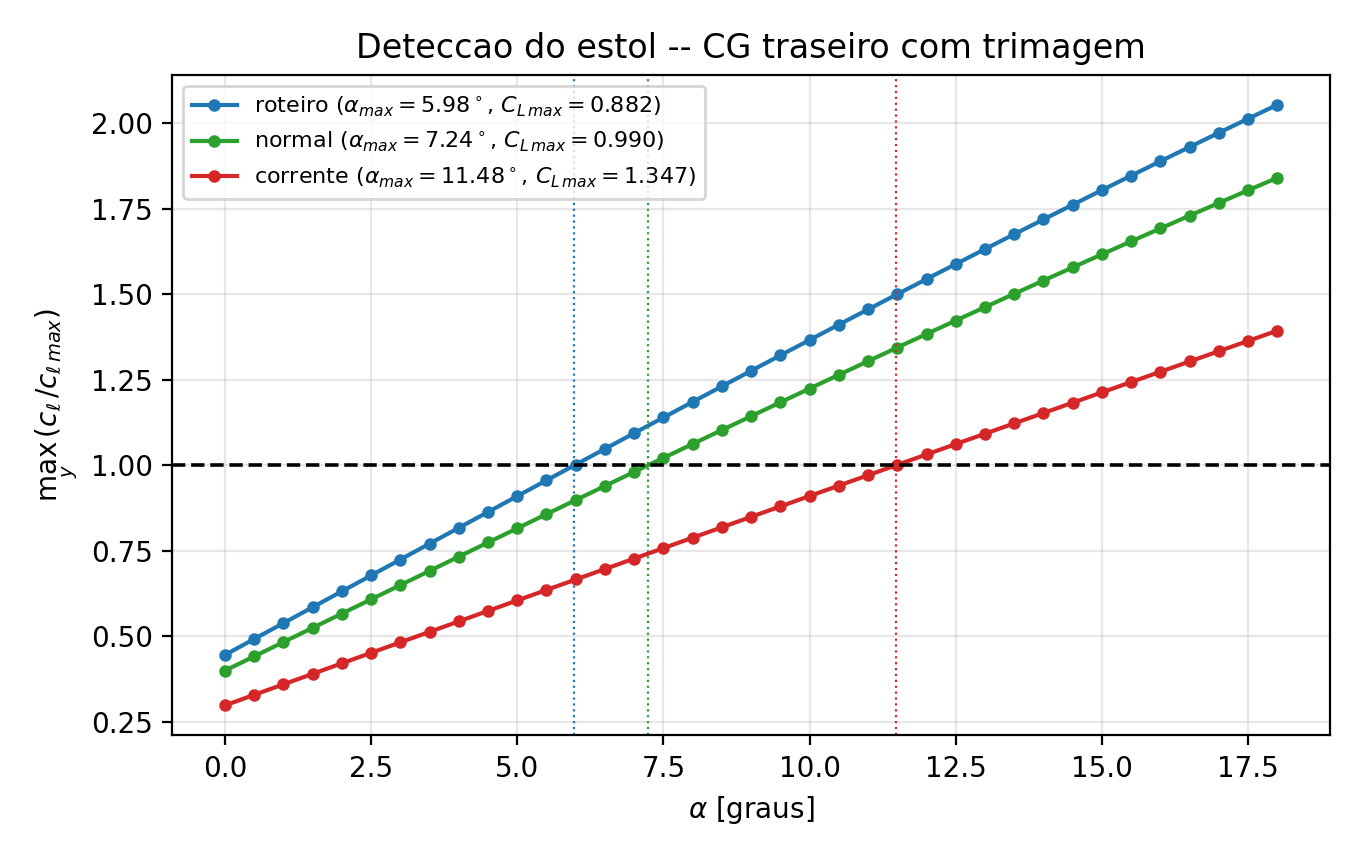
\includegraphics[width=0.66\textwidth]{resultados_q4/deteccao_estol.png}
\caption{Detecção do estol: carregamento máximo da seção em função de $\alpha$
para os três critérios, no caso de CG traseiro com trimagem.}
\label{fig:deteccao}
\end{figure}

\subsection{Resultados}

A Tab.~\ref{tab:secao-critica} reúne os quatro casos pedidos pelo enunciado. As
distribuições de sustentação na condição de estol estão na
Fig.~\ref{fig:cl-y-estol}, com a curva de limite de $c_{\ell\,max}$ sobreposta,
e a Fig.~\ref{fig:razao} mostra o grau de carregamento
$c_\ell/c_{\ell\,max}$ de cada seção.

\begin{table}[H]
\centering
\caption{$\alpha_{max}$, $C_{L\,max}$ e deflexão de profundor de asa limpa em
baixa velocidade ($M=\scMach$), pelo método da seção crítica. A última coluna dá
a estação $\eta=y/(b/2)$ em que o estol começa.}
\label{tab:secao-critica}
\begin{tabular}{lccccc}
\toprule
Caso & $i_t$ [$^\circ$] & $\alpha_{max}$ [$^\circ$] & $C_{L\,max}$ & $\delta_e$ [$^\circ$] & $\eta$ do estol \\
\midrule
CG dianteiro, sem trimagem & $-3.429$ & 5.98 & 0.864 & $+0.00$ & 0.907 \\
CG dianteiro, com trimagem & $-3.429$ & 5.99 & 0.854 & $-1.95$ & 0.907 \\
CG traseiro, sem trimagem & $-1.959$ & 5.98 & 0.877 & $+0.00$ & 0.907 \\
CG traseiro, com trimagem & $-1.959$ & 5.98 & 0.882 & $+0.97$ & 0.907 \\
\bottomrule
\end{tabular}

\end{table}

\begin{figure}[H]
\centering
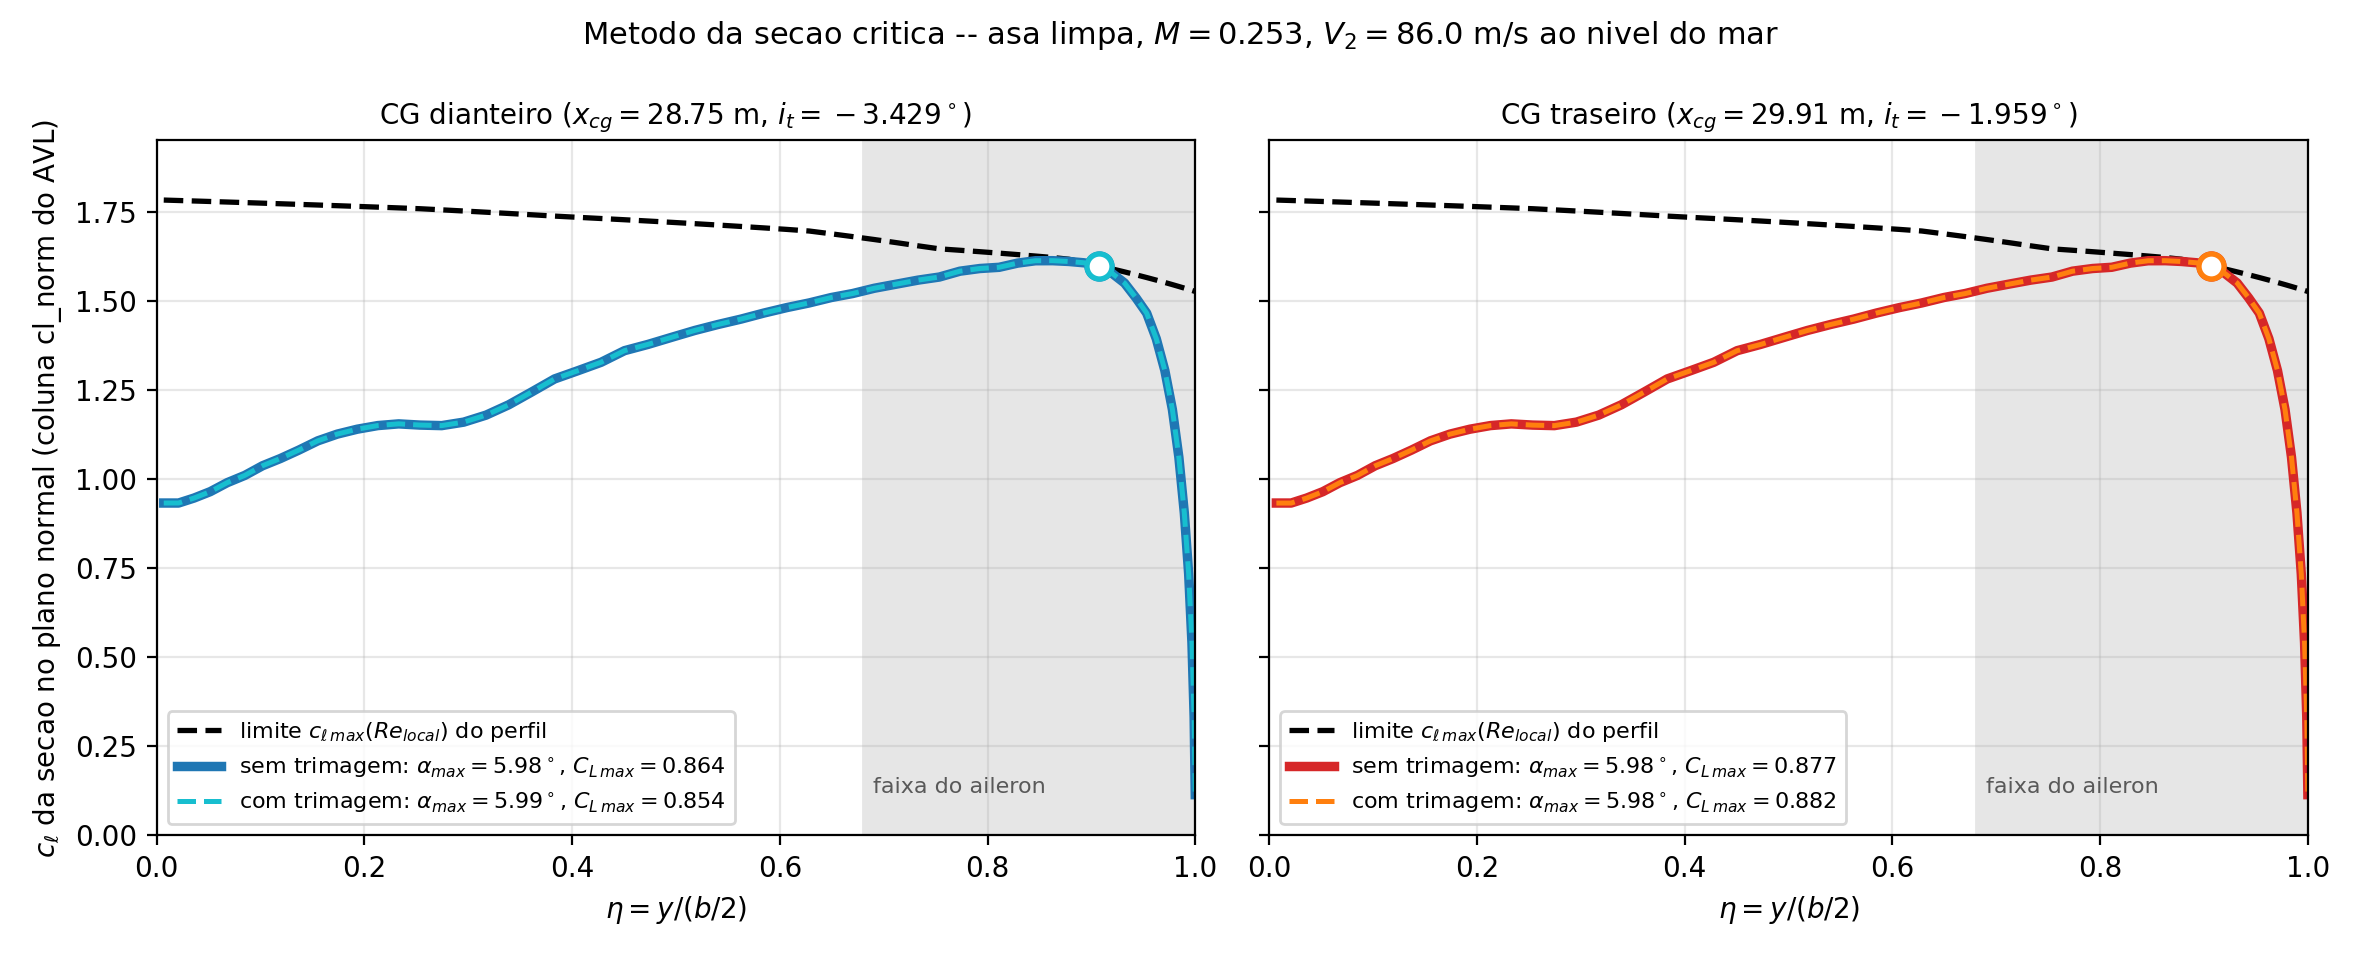
\includegraphics[width=\textwidth]{resultados_q4/cl_y_estol.png}
\caption{Distribuições de $c_\ell$ (coluna \code{cl\_norm}) na condição de
estol, para as duas posições de CG, com e sem trimagem. A linha tracejada é o
limite $c_{\ell\,max}(Re_{local})$ do perfil; o círculo marca a seção crítica.}
\label{fig:cl-y-estol}
\end{figure}

\begin{figure}[H]
\centering
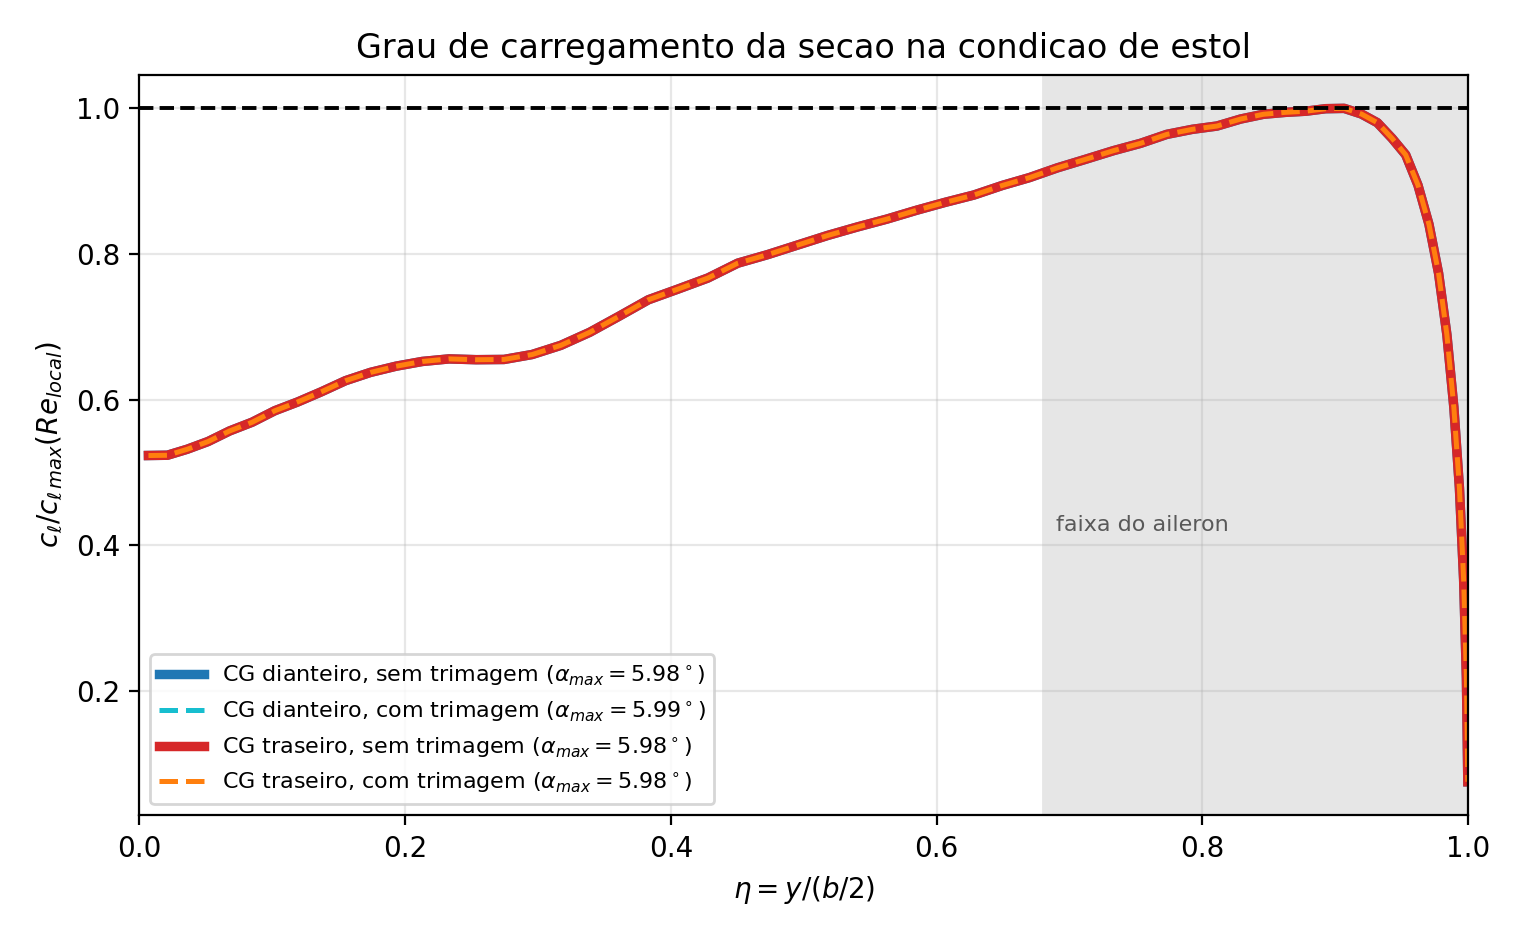
\includegraphics[width=0.72\textwidth]{resultados_q4/razao_cl_clmax.png}
\caption{Grau de carregamento das seções na condição de estol. O estol começa
onde a curva toca a unidade.}
\label{fig:razao}
\end{figure}

\begin{table}[H]
\centering
\caption{Sensibilidade do $C_{L\,max}$ à leitura do critério de estol (casos
trimados). O valor do \code{designTool} é a correlação empírica
$0{,}9\,c_{\ell\,max}\cos\Lambda$ usada em \code{aerodynamics.py}.}
\label{tab:criterios}
\begin{tabular}{lcccc}
\toprule
Criterio de estol & \multicolumn{2}{c}{CG dianteiro} & \multicolumn{2}{c}{CG traseiro} \\
& $\alpha_{max}$ [$^\circ$] & $C_{L\,max}$ & $\alpha_{max}$ [$^\circ$] & $C_{L\,max}$ \\
\midrule
roteiro: $c_\ell^{\,norm}$ vs.\ perfil da corrente & 5.99 & 0.854 & 5.98 & 0.882 \\
coerente: $c_\ell^{\,norm}$ vs.\ perfil do plano normal & 7.25 & 0.958 & 7.24 & 0.990 \\
sem correcao: $c_\ell$ vs.\ perfil da corrente & 11.49 & 1.304 & 11.48 & 1.347 \\
\bottomrule
\end{tabular}

\end{table}

\subsection{Discussão}

\paragraph{Efeito da posição de CG e da trimagem.}
O $\alpha_{max}$ é praticamente o mesmo nos quatro casos
($\approx \scAlphaAftTrim^\circ$, com variação inferior a $0{,}02^\circ$ entre
eles), o que era esperado: o
estol é ditado pela distribuição de sustentação da asa, que depende de $\alpha$
e quase não sente o profundor. O que muda é o $C_{L\,max}$ da \emph{aeronave}.
Sem trimagem, a empenagem com $i_t$ negativo já produz uma carga para baixo
fixa, e o CG traseiro dá $C_{L\,max}=\scCLmaxAftLivre$ contra
$\scCLmaxFwdLivre$ do CG dianteiro --- a diferença vem inteiramente do $i_t$
menos negativo que o CG traseiro permite ($\scItAft^\circ$ contra
$\scItFwd^\circ$).

Com a restrição de trimagem, o profundor tem de gerar o momento que falta para
$C_M=0$ no ângulo de estol, e aí os dois CGs se comportam de forma oposta:

\begin{itemize}
  \item no \textbf{CG dianteiro} a aeronave ainda está com o nariz pesado no
  ângulo de estol; o profundor sobe ($\delta_e = \scDeFwdTrim^\circ$), acrescenta
  carga descendente na empenagem e o $C_{L\,max}$ \emph{cai} de
  $\scCLmaxFwdLivre$ para $\scCLmaxFwdTrim$;
  \item no \textbf{CG traseiro} o sinal se inverte: a margem estática é pequena
  e, com $i_t$ pouco negativo, sobra momento de cabrar no estol. O profundor
  desce ($\delta_e = \scDeAftTrim^\circ$), acrescenta sustentação, e o
  $C_{L\,max}$ \emph{sobe} de $\scCLmaxAftLivre$ para $\scCLmaxAftTrim$.
\end{itemize}

Vale notar que essa inversão é consequência direta da escolha de $i_w$ feita no
item~3: com a asa a $\scIw^\circ$ e o $i_t$ reajustado, o ângulo de estol caiu
para perto de $6^\circ$ de fuselagem e o equilíbrio de momentos ali mudou de
lado no CG traseiro. \textbf{O caso crítico para o dimensionamento é o CG
dianteiro com trimagem}, com $C_{L\,max} = \scCLmaxFwdTrim$ --- é esse o valor
que deve alimentar as contas de velocidade de estol, comprimento de pista e
distância de pouso.

\paragraph{Onde o estol começa: o ponto fraco do projeto.}
Nos quatro casos a seção crítica fica em $\eta = \scEtaAftTrim$, isto é,
\textbf{dentro da faixa do aileron}, que vai de $\eta=\scEtaAil$ à ponta. Isso é
inadequado: o estol começa justamente onde está a superfície de controle de
rolamento, com três consequências ruins:
\begin{enumerate}
  \item perda de autoridade de rolamento no momento em que ela é mais
  necessária, com risco de rolamento assimétrico se a separação começar antes
  em uma semi-asa;
  \item ausência de aviso de estol aerodinâmico --- a esteira separada não passa
  pela empenagem nem pela fuselagem, de modo que não há \emph{buffet} natural
  para avisar o piloto;
  \item tendência de momento de arfagem para cima (\emph{pitch-up}): a perda de
  sustentação na ponta de uma asa enflechada ocorre atrás do CG, o que agrava o
  estol em vez de aliviá-lo.
\end{enumerate}

Pior: a Fig.~\ref{fig:razao} mostra que a razão $c_\ell/c_{\ell\,max}$ fica
acima de $0{,}97$ em toda a faixa
$\scEtaPlatIni \leq \eta \leq \scEtaPlatFim$. Não se trata de uma seção isolada
tocando o limite, mas de um quinto externo de semi-asa inteiro a menos de 3\%
do estol --- o que significa separação abrupta e ao mesmo tempo em toda essa
extensão, em vez da propagação gradual que dá aviso ao piloto.

A causa é geométrica e está clara na Fig.~\ref{fig:razao}: o afilamento
$\lambda = \scAfilamento$ é muito agressivo (o usual em transportes é
$0{,}25$--$0{,}35$) e os modelos AVL do grupo têm \textbf{torção nula}. A
combinação empurra o carregamento para fora --- na seção crítica
$c_\ell/C_L = \scFatorCarga$ --- e, como o Reynolds local na ponta é cinco vezes
menor que na raiz, o limite de $c_{\ell\,max}$ ainda cai de $\scClmaxRaiz$ para
$\scClmaxPonta$ exatamente onde a carga é maior. Os dois efeitos se somam na
direção errada.

A correção clássica é torção geométrica negativa (\emph{washout}) de
$3^\circ$ a $4^\circ$ na ponta, que redistribui a carga para dentro e desloca a
seção crítica para $\eta \approx 0{,}4$--$0{,}6$. Vale notar que o \code{slat}
projetado vai até $\eta = \scEtaSlat$ e, portanto, protege a região crítica nas
configurações de decolagem e pouso; o problema descrito aqui é da
\textbf{asa limpa}, que é a condição de estol em cruzeiro e em manobra. A
recomendação para o grupo é reintroduzir torção nos arquivos \code{.avl} e no
\code{designTool} antes de fechar o projeto.

\paragraph{Comparação com o \code{designTool}.}
O \code{designTool} estima o $C_{L\,max}$ de asa limpa pela correlação empírica
$C_{L\,max} = 0{,}9\,c_{\ell\,max}\cos\Lambda = \scCLmaxDT$. O método da seção
crítica, com o critério do roteiro, dá \scRazaoDT\% desse valor. A discrepância
não é erro de conta: ela mede a distância entre uma correlação calibrada para
asas bem torcidas e a asa que o grupo realmente desenhou. A
Tab.~\ref{tab:criterios} mostra que a leitura sem correção de enflechamento
($C_{L\,max} = \scCLmaxCorrAftTrim$) fica do outro lado do valor do
\code{designTool}, e a versão coerente da teoria de enflechamento simples
($\scCLmaxNormAftTrim$) fica entre as duas. Ou seja: o valor do
\code{designTool} está dentro da faixa de incerteza do método, mas no extremo
otimista dela. Como todo o dimensionamento de pista depende do $C_{L\,max}$,
convém tratar $\scCLmaxFwdTrim$ como o valor conservador de projeto e refazer a
restrição de pouso do Lab~02 com ele, além de adotar a torção discutida acima.

\paragraph{Limitações do modelo.}
Três simplificações devem ser lembradas na leitura dos números: (i) o AVL é um
método de painéis potencial e não modela separação --- o método da seção crítica
é um critério externo aplicado sobre um campo linear, e por isso superestima a
sustentação perto do estol; (ii) os arquivos \code{.avl} usam um único
\code{AFILE} em todas as estações, enquanto a asa real varia de
$t/c=\scTcRaiz$ na raiz a $\scTcPonta$ na ponta, de forma que o limite de
$c_{\ell\,max}$ na ponta é provavelmente otimista; (iii) o $c_{\ell\,max}$ do
XFOIL para este perfil tem incerteza numérica da ordem de $\pm 0{,}03$ (medida
no Lab~03 variando painéis e passo de $\alpha$), o que se traduz em cerca de
$\pm 0{,}015$ no $C_{L\,max}$ da aeronave.

% =====================================================================
% Lab 04 --- Item 2.5: polares de arrasto
% Incluido por main.tex. Tabelas em tex_q5/ e figuras em
% resultados_q5/ (mesmo nivel que este arquivo e o main.tex).
% Codigos em polares/.
% =====================================================================
% gerado por q5_polares.py
\newcommand{\poAlphaAftLivre}{0.04}
\newcommand{\poAlphaAftTrim}{0.04}
\newcommand{\poAlphaFwdLivre}{0.18}
\newcommand{\poAlphaFwdTrim}{0.18}
\newcommand{\poAlt}{10668}
\newcommand{\poCDAftLivre}{0.02023}
\newcommand{\poCDAftTrim}{0.02023}
\newcommand{\poCDFwdLivre}{0.02081}
\newcommand{\poCDFwdTrim}{0.02081}
\newcommand{\poCDaFit}{0.18763}
\newcommand{\poCDaaFit}{1.48578}
\newcommand{\poCDdt}{0.02183}
\newcommand{\poCDzeroDT}{0.01328}
\newcommand{\poCDzeroFit}{0.02010}
\newcommand{\poCLmaxAftLivre}{0.877}
\newcommand{\poCLmaxAftTrim}{0.882}
\newcommand{\poCLmaxFwdLivre}{0.864}
\newcommand{\poCLmaxFwdTrim}{0.854}
\newcommand{\poCLmin}{-0.5}
\newcommand{\poCLproj}{0.4702}
\newcommand{\poDeAftLivre}{+0.00}
\newcommand{\poDeAftTrim}{+0.00}
\newcommand{\poDeFwdLivre}{+0.00}
\newcommand{\poDeFwdTrim}{-0.00}
\newcommand{\poDifAbsAftLivre}{7.3}
\newcommand{\poDifAbsAftTrim}{7.3}
\newcommand{\poDifAbsFwdLivre}{4.7}
\newcommand{\poDifAbsFwdTrim}{4.7}
\newcommand{\poDifAftLivre}{-7.3}
\newcommand{\poDifAftTrim}{-7.3}
\newcommand{\poDifFwdLivre}{-4.7}
\newcommand{\poDifFwdTrim}{-4.7}
\newcommand{\poEffAftLivre}{23.2}
\newcommand{\poEffAftTrim}{23.2}
\newcommand{\poEffDT}{21.5}
\newcommand{\poEffFwdLivre}{22.6}
\newcommand{\poEffFwdTrim}{22.6}
\newcommand{\poItAft}{-1.959}
\newcommand{\poItFwd}{-3.429}
\newcommand{\poIw}{4.5}
\newcommand{\poMach}{0.85}
\newcommand{\poRdois}{0.99999}


\section{Item 5 --- Polares de arrasto}
\label{sec:polares}

\subsection{Montagem das curvas}

As quatro polares pedidas pelo enunciado foram levantadas no Mach e na altitude
do ponto de projeto ($M = \poMach$, $h = \poAlt$~m), com a incidência de
empenagem do item~3 e todas as superfícies de alta sustentação neutras:

\begin{enumerate}[label=(\alph*)]
  \item CG dianteiro sem deflexões de superfície de controle
  ($\delta_e$ travado em zero);
  \item CG traseiro sem deflexões de superfície de controle;
  \item CG dianteiro com arfagem compensada ($C_M = 0$);
  \item CG traseiro com arfagem compensada ($C_M = 0$).
\end{enumerate}

Em vez de varrer $\alpha$ e depois recortar, usou-se diretamente a restrição de
$C_L$ do AVL (comando \code{a c}), o que faz cada curva nascer e morrer
exatamente onde o enunciado pede: de $C_L = \poCLmin$ até o $C_{L\,max}$
calculado pelo método da seção crítica no item~4, que é específico de cada
caso (Tab.~\ref{tab:secao-critica}). Nos casos (a) e (b) o profundor é travado
em zero (\code{d4 d4 0}); nos casos (c) e (d) entra a restrição de trimagem
(\code{d4 pm 0}). O ponto de projeto foi incluído na grade de $C_L$ para ser
lido sem interpolação.

\subsection{Resultados}

A Fig.~\ref{fig:polar} traz as quatro polares em um único gráfico, junto com a
polar do \code{designTool} na mesma condição, e a Fig.~\ref{fig:polar-zoom}
amplia a vizinhança do ponto de projeto, onde as curvas se distinguem.

\begin{figure}[H]
\centering
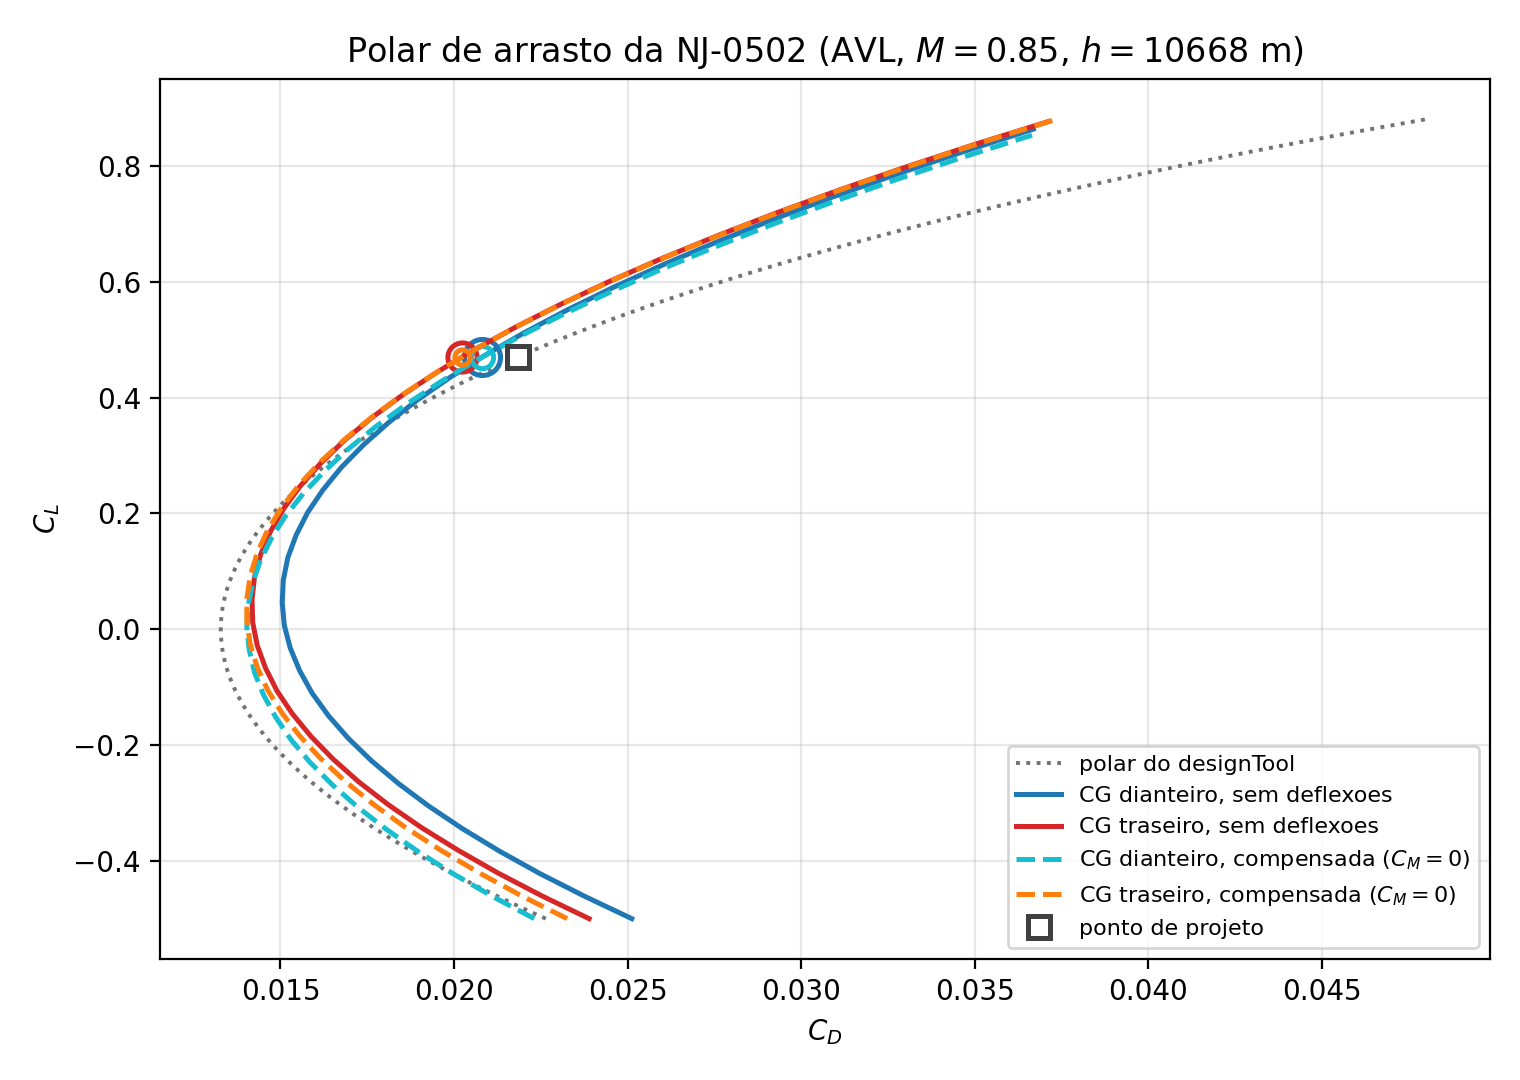
\includegraphics[width=0.74\textwidth]{resultados_q5/polar_CD_CL.png}
\caption{Polares de arrasto da NJ-0502 no ponto de projeto
($M=\poMach$, $h=\poAlt$~m). Cada curva termina no $C_{L\,max}$ do item~4.
Os círculos marcam o ponto de projeto ($C_L = \poCLproj$) e o quadrado, o ponto
de projeto segundo a polar do \code{designTool}.}
\label{fig:polar}
\end{figure}

\begin{figure}[H]
\centering
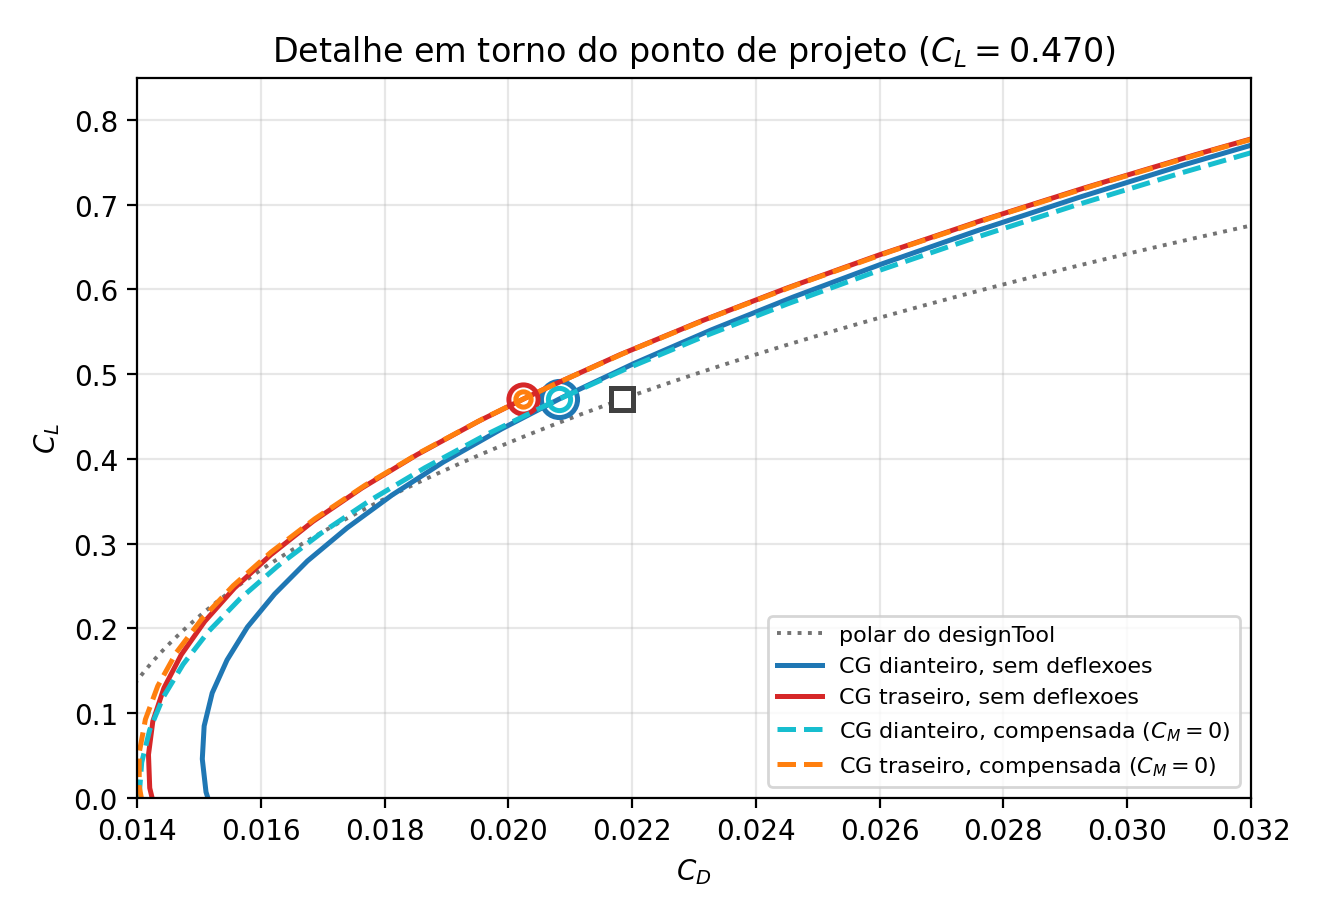
\includegraphics[width=0.7\textwidth]{resultados_q5/polar_CD_CL_zoom.png}
\caption{Detalhe das polares em torno do ponto de projeto.}
\label{fig:polar-zoom}
\end{figure}

\begin{table}[H]
\centering
\caption{$C_D$ no $C_L$ do ponto de projeto ($C_L = \poCLproj$) para as quatro
configurações, comparado com o valor da polar do \code{designTool}.}
\label{tab:CD-ponto}
\begin{tabular}{lccccc}
\toprule
Configuracao & $\alpha$ [$^\circ$] & $\delta_e$ [$^\circ$] & $C_D$ (AVL) & $C_D$ (designTool) & dif. \\
\midrule
CG dianteiro, sem deflexoes & 0.18 & $+0.00$ & 0.02081 & 0.02183 & $-4.7$\% \\
CG traseiro, sem deflexoes & 0.04 & $+0.00$ & 0.02023 & 0.02183 & $-7.3$\% \\
CG dianteiro, compensada ($C_M=0$) & 0.18 & $+0.00$ & 0.02081 & 0.02183 & $-4.7$\% \\
CG traseiro, compensada ($C_M=0$) & 0.04 & $+0.00$ & 0.02023 & 0.02183 & $-7.3$\% \\
\bottomrule
\end{tabular}

\end{table}

\subsection{Discussão}

\paragraph{Efeito do CG e da trimagem no ponto de projeto.}
As quatro configurações praticamente coincidem no ponto de projeto:
$C_D = \poCDFwdLivre$ no CG dianteiro e $\poCDAftLivre$ no CG traseiro, com
diferença desprezível entre as versões trimada e não trimada
($\delta_e = \poDeFwdTrim^\circ$ e $\poDeAftTrim^\circ$). Isso não é
coincidência: é a verificação numérica do item~3. O $i_t$ de cada arquivo foi
escolhido justamente para anular o profundor nesse $C_L$, de modo que trimar ou
não trimar dá o mesmo resultado \emph{ali}. A separação entre as curvas cheias e
tracejadas na Fig.~\ref{fig:polar} cresce à medida que se afasta do ponto de
projeto, e é onde aparece o arrasto de trimagem.

A pequena vantagem do CG traseiro ($\poDifAftLivre$\% contra
$\poDifFwdLivre$\% em relação ao \code{designTool}) tem a mesma origem: com o CG
mais atrás, o $i_t$ necessário é menos negativo ($\poItAft^\circ$ contra
$\poItFwd^\circ$), a carga descendente na empenagem é menor e a asa precisa
gerar menos sustentação --- logo menos arrasto induzido. É o argumento clássico
a favor de voar com o CG o mais atrás que a margem estática permitir.

\paragraph{Comparação com a polar do \code{designTool}.}
O AVL fica \poDifAbsAftLivre\% \emph{abaixo} do \code{designTool}
($C_D = \poCDdt$) no ponto de projeto, o que corresponde a uma eficiência
$C_L/C_D$ de \poEffAftLivre{} contra \poEffDT{}. A diferença tem duas origens
identificáveis:

\begin{itemize}
  \item o \textbf{arrasto parasita é o mesmo por construção}: o campo
  \code{\# CDp} dos arquivos \code{.avl} recebeu o próprio $C_{D0}$ de cruzeiro
  do \code{designTool} ($\poCDzeroDT$), e o AVL o devolve intacto na linha
  \code{CDvis}. Não há divergência a explicar aqui;
  \item a diferença está toda no \textbf{arrasto induzido e de onda}. O AVL
  resolve a distribuição de sustentação da asa real e obtém um fator de
  Oswald próprio, enquanto o \code{designTool} usa a correlação
  $C_{D} = C_{D0} + K C_L^{2}$ com um $K$ que já embute uma parcela de arrasto de
  onda em $M = \poMach$. Como o AVL é um método potencial linear, ele
  \emph{não modela arrasto de onda nenhum} --- e é exatamente essa parcela que
  falta.
\end{itemize}

A conclusão prática é que as duas estimativas não são substituíveis: o AVL é
melhor para o arrasto induzido e para capturar o efeito de CG e de trimagem,
mas subestima o arrasto total em cruzeiro transônico. Para o desempenho da
aeronave em $M = \poMach$ o valor do \code{designTool} continua sendo o
mais adequado; a contribuição do AVL aqui é mostrar que a parcela induzida está
bem estimada e quantificar o custo de trimagem fora do ponto de projeto.

\paragraph{Ajuste quadrático para a Seção~3 (Tab.~7 do enunciado).}
A polar não trimada de CG traseiro (caso 5.b) foi ajustada por
$C_D = C_{D0} + C_{D\alpha}\,\alpha + C_{D\alpha^{2}}\,\alpha^{2}$, com $\alpha$
em radianos, na faixa de $C_L$ de $-0{,}1$ ao $C_{L\,max}$
(Fig.~\ref{fig:ajuste} e Tab.~\ref{tab:ajuste}). O ajuste é excelente
($R^{2} = \poRdois$), como era de esperar de uma polar essencialmente
parabólica.

\textbf{Atenção: o $C_{D0}$ deste ajuste não é o arrasto parasita.} O termo
constante vale $\poCDzeroFit$, bem acima do $C_{D0}$ de $\poCDzeroDT$ que foi
\emph{dado} ao AVL no campo \code{\# CDp}. Não há contradição --- são grandezas
diferentes. Como a asa está a $i_w = \poIw^\circ$ (item~3), $\alpha = 0$ é a
atitude de \emph{fuselagem nivelada}, que é praticamente o próprio ponto de
projeto: ali o avião já gera $C_L \approx \poCLproj$ e, com ele, todo o arrasto
induzido correspondente. Por isso $\poCDzeroFit \approx \poCDAftLivre$, o $C_D$
do ponto de projeto.

Essa é exatamente a forma que o modelo de MVO espera, porque lá o $\alpha$
também é medido a partir da linha de referência da fuselagem. O preço é que o
termo linear deixa de ser desprezível: $C_{D\alpha} = \poCDaFit$/rad, contra um
valor quase nulo que se obteria se $\alpha$ fosse contado da sustentação nula.
Ao transcrever a Tab.~\ref{tab:ajuste} para a Seção~3, portanto, é preciso usar
os três coeficientes juntos --- o $C_{D0}$ isolado não tem o significado de
arrasto parasita.

\begin{figure}[H]
\centering
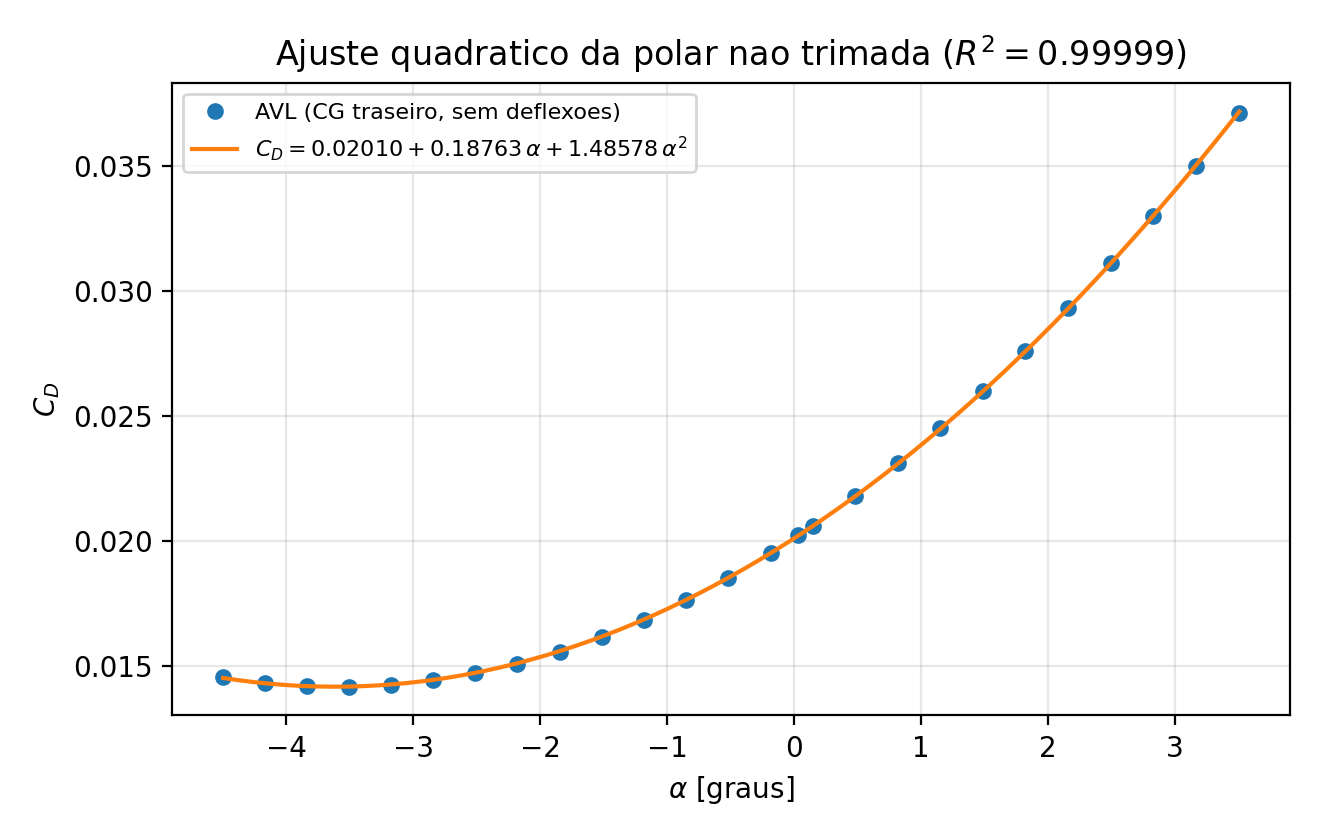
\includegraphics[width=0.68\textwidth]{resultados_q5/ajuste_CD_alpha.png}
\caption{Ajuste quadrático da polar não trimada de CG traseiro, usado para
preencher a Tab.~7 do enunciado.}
\label{fig:ajuste}
\end{figure}

\begin{table}[H]
\centering
\caption{Ajuste quadrático da polar de arrasto não trimada (exercício 5.b).}
\label{tab:ajuste}
\begin{tabular}{llr}
\toprule
Parametro & Explicacao & Valor \\
\midrule
$C_{D0}$ & termo constante ($\alpha$ da fuselagem; nao e o arrasto parasita) & 0.02010 \\
$C_{D\alpha}$ & termo linear [1/rad] & 0.18763 \\
$C_{D\alpha^2}$ & termo quadratico [1/rad$^2$] & 1.48578 \\
\bottomrule
\end{tabular}

\end{table}

\paragraph{Faixa de validade das curvas.}
Como cada polar termina no $C_{L\,max}$ de baixa velocidade do item~4, os
trechos de $C_L$ alto das curvas da Fig.~\ref{fig:polar} são formalmente
inconsistentes: eles estão traçados em $M = \poMach$, condição em que a
aeronave nunca chegaria a $C_L = \poCLmaxAftLivre$ sem antes entrar em estol de
onda (\emph{shock stall}), bem antes do estol de bordo de ataque calculado no
item~4. O corte foi mantido porque é o que o enunciado pede, mas na prática
apenas a região $0{,}3 \lesssim C_L \lesssim 0{,}6$ dessas curvas representa
condições de voo realizáveis em cruzeiro. Os arquivos
\code{resultados\_q5/polar\_*.csv} guardam $\alpha$, $\delta_e$ e $C_M$ de
cada ponto, o que permite refazer as curvas em outra condição sem rodar o AVL
de novo.


\end{document}
